% =========================================================
\chapter{Lecture 4 : Mandatory Access Control}
% =========================================================

\begin{rembox}[title=In a nutshell]
\textbf{What is this lecture about?} In \textbf{MAC}, it is not the owner but a
\textbf{central policy} that decides, and nobody can override it. We study three classic
``recipes'' (security models): \textbf{Bell-La Padula} to keep secrets from leaking down
(army: no read up, no write down), \textbf{BIBA} to keep bad data from corrupting good
data (bank: no read down, no write up), and the \textbf{Chinese Wall} to avoid conflicts
of interest (a consultant cannot work for Pepsi and Coca-Cola). \\
\textbf{Why is it useful?} When an organization must guarantee a property no matter what
users do (military secrets, bank records, hospitals), these models give a ready-made,
proven design. They also explain deep real-world problems: hidden leaks (\emph{covert
channels}), why declassifying documents is hard, and why unchecked user input
(\emph{sanitization}) causes SQL injections and buffer overflows.
\end{rembox}

\begin{defnbox}[title=Mandatory Access Control (MAC)]
Access to and operations on resources \textbf{are determined by the security policy}
(a central security policy assigns permissions):
\begin{itemize}
  \item the ``owner'' may not exist, or may not have the power to set permissions
        against the policy;
  \item the security policy \textbf{must} be enforced despite subjects trying to
        subvert it.
\end{itemize}
\end{defnbox}

\begin{rembox}[title=Reminder: DAC vs.\ MAC]
In DAC, owners have all powers on the objects they create. In MAC, the policy is given: there may
be no ``object owners'' at all, and even the creator of an object cannot set its permissions,
only assign the rights dictated by the policy. (A theoretical lecture: concepts that outlast
technology.)
\end{rembox}

\begin{defnbox}[title=Security model]
A \textbf{design pattern} for a specific security property or set of properties. When
faced with a standard security problem $\to$ use a well-known model! \\
A model is \textbf{not} a policy nor a mechanism: it is a way of reasoning to build policies that
ensure the properties. The details of the policy must still be defined by the engineer, and
following the pattern carelessly does not guarantee security.
\end{defnbox}

\begin{warnbox}[title=The devil is in the details]
Many aspects are \textbf{not covered by the model}: who are the subjects? what are the
objects? what mechanisms to use to implement it?
\end{warnbox}

\begin{goatbox}
In MAC the farm's rule book decides, not the goats. Rather than inventing a rule book from
scratch, you copy a well-known recipe (a model) made for your problem: one recipe for keeping
secrets, one for keeping things clean, one for not working for two rivals. The recipe tells the
shape of the rules; you still have to decide who the goats and buckets are.
\end{goatbox}

\section{Bell-La Padula (BLP): protecting confidentiality}

\begin{defnbox}[title=Bell-La Padula model (BLP)]
Subjects $S$ and objects $O$ are associated to a \textbf{level} of confidentiality.
Subjects' access rights are defined (in an access control matrix) by four attributes:
\begin{itemize}
  \item \textbf{Execute} --- the subject cannot see or modify the object, but can run it;
  \item \textbf{Read} --- the subject can only see the object but cannot modify it;
  \item \textbf{Append} --- the subject cannot read the object, but can attach new
        content;
  \item \textbf{Write} --- the subject can see the object and add content or modify
        existing content.
\end{itemize}
\end{defnbox}

\begin{rembox}[title=Observe vs.\ alter]
\textbf{Observe} rights: read ($r$), write ($w$). \textbf{Alter} rights: append ($a$),
write ($w$). Write is both observe and alter.
\end{rembox}

\begin{defnbox}[title=State of a BLP system]
At any time, the state is: (1) the \textbf{levels} of subjects (clearance) and objects
(classification); (2) the \textbf{access control matrix} giving the attributes of each subject on
each object; (3) the \textbf{current accesses} (which subject accesses which object with which
right) authorized at that time.
\end{defnbox}

\subsection{Security levels and dominance}

\begin{defnbox}[title=Security level (classification of objects)]
Objects are associated to a \textbf{security level}: they have a \textbf{label} and
belong to one or more \textbf{categories}.
\[
  \text{Security level} = (\text{Classification}, \{\text{set of categories}\})
\]
\begin{itemize}
  \item \textbf{Classification} --- \textbf{total order} of labels (e.g.\
        Unclassified $<$ Confidential $<$ Secret $<$ Top Secret).
  \item \textbf{Categories} --- compartments of objects with a common topic (e.g.\
        Nuclear, NATO, Crypto).
\end{itemize}
\end{defnbox}

\begin{defnbox}[title=Dominance relationship]
A security level $(l_1, c_1)$ \textbf{dominates} $(l_2, c_2)$ \textbf{if and only if}
\[
  l_1 \geq l_2 \quad\text{and}\quad c_2 \subseteq c_1 .
\]
\end{defnbox}

\begin{exbox}[title={Exercise --- Dominance}]
Labels: Admin $<$ Nurse $<$ Surgeon $<$ Doctor; categories: DEMOGRAPHICS, ANALYSIS,
RESULTS. Which statements are true?
\begin{itemize}
  \item $(D, \{\})$ dominates $(S, \{\})$
  \item $(S, \{\})$ dominates $(N, \{\text{RESULTS}\})$
  \item $(S, \{\text{DEMOGRAPHICS}, \text{RESULTS}\})$ dominates
        $(N, \{\text{DEMOGRAPHICS}\})$
  \item $(D, \{\text{ANALYSIS}, \text{RESULTS}\})$ dominates
        $(S, \{\text{DEMOGRAPHICS}\})$
\end{itemize}
What level dominates them all? What level dominates only itself? \\[3pt]
\textbf{Solution.}
\begin{itemize}
  \item $(D, \{\})$ dom.\ $(S, \{\})$: \textbf{true} (Doctor $>$ Surgeon, $\{\} \subseteq \{\}$).
  \item $(S, \{\})$ dom.\ $(N, \{\text{RESULTS}\})$: \textbf{false}: S $>$ N, but this nurse sees
        RESULTS and the surgeon does not ($\{\text{RESULTS}\} \not\subseteq \{\}$).
  \item $(S, \{\text{DEM}, \text{RES}\})$ dom.\ $(N, \{\text{DEM}\})$: \textbf{true} (higher label,
        and more categories).
  \item $(D, \{\text{ANA}, \text{RES}\})$ dom.\ $(S, \{\text{DEM}\})$: \textbf{false}: higher
        label, but the surgeon sees DEMOGRAPHICS (different information): no relation.
\end{itemize}
Top (dominates all): $(\text{Doctor}, \{\text{DEMOGRAPHICS}, \text{ANALYSIS},
\text{RESULTS}\})$. Bottom (dominates only itself): $(\text{Admin}, \{\})$.
\end{exbox}

\begin{goatbox}
Each paper gets a stamp: a height (how secret) and a set of colours (which topics). You may look
at a paper only if your badge is at least as high \emph{and} has all the paper's colours. A
higher badge with a missing colour is not enough: a general without the ``Nuclear'' colour cannot
read a Nuclear paper.
\end{goatbox}

\begin{propbox}[title=Dominance lattice]
Three key properties:
\begin{enumerate}[label=(\alph*)]
  \item dominates is \textbf{transitive};
  \item there are \textbf{top and bottom} elements;
  \item it is only a \textbf{partial} order: two levels may be incomparable (e.g.\
        $(S, \{\text{Crypto}\})$ and $(S, \{\text{Nuclear}\})$).
\end{enumerate}
\begin{center}
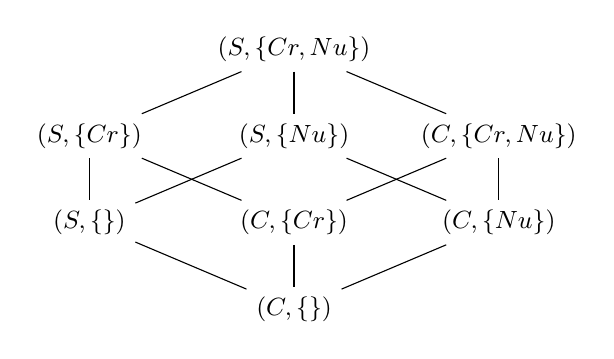
\begin{tikzpicture}[x=2.6cm, y=1.1cm, every node/.style={font=\small}]
  \node (top) at (0,3)    {$(S, \{Cr, Nu\})$};
  \node (sc)  at (-1,2)   {$(S, \{Cr\})$};
  \node (sn)  at (0,2)    {$(S, \{Nu\})$};
  \node (ccn) at (1,2)    {$(C, \{Cr, Nu\})$};
  \node (s0)  at (-1,1)   {$(S, \{\})$};
  \node (cc)  at (0,1)    {$(C, \{Cr\})$};
  \node (cn)  at (1,1)    {$(C, \{Nu\})$};
  \node (bot) at (0,0)    {$(C, \{\})$};
  \draw (top) -- (sc); \draw (top) -- (sn); \draw (top) -- (ccn);
  \draw (sc) -- (s0);  \draw (sn) -- (s0);
  \draw (sc) -- (cc);  \draw (sn) -- (cn);
  \draw (ccn) -- (cc); \draw (ccn) -- (cn);
  \draw (s0) -- (bot); \draw (cc) -- (bot); \draw (cn) -- (bot);
\end{tikzpicture} \\
{\small Labels $C < S$, categories Crypto, Nuclear: a higher node dominates every node
reachable downwards.}
\end{center}
Transitivity example: $(S, \{Cr, Nu\})$ dom.\ $(S, \{Nu\})$ and $(S, \{Nu\})$ dom.\ $(C,
\{Nu\})$, so $(S, \{Cr, Nu\})$ dom.\ $(C, \{Nu\})$. No relation: $(S, \{Nu\})$ and $(S,
\{Cr\})$.
\end{propbox}

\begin{defnbox}[title=Clearance of subjects]
\begin{itemize}
  \item \textbf{Clearance} --- maximum security level a subject has been assigned:
        $\text{level}(S_i)$ (BLP also calls this ``classification'').
  \item \textbf{Current security level} --- subjects can operate at lower security
        levels: $\text{current-level}(S_i)$.
\end{itemize}
$\text{level}(S_i)$ \textbf{must dominate} $\text{current-level}(S_i)$!
\end{defnbox}

\subsection{The three BLP properties}

\begin{defnbox}[title=Simple security property (ss-property) --- No Read Up]
If (subject, object, $r$) is a current access, then $\text{level}(\text{subject})$
\textbf{dominates} $\text{level}(\text{object})$. \\
$\Rightarrow$ \textbf{No Read Up (NRU)}: a subject cleared Secret can read Secret,
Classified, Unclassified, but not Top Secret.
\end{defnbox}

\begin{warnbox}[title=Why is the ss-property not sufficient?]
A Secret subject runs \textbf{malicious code} (Trojan) that reads Secret data (allowed
by NRU) and \textbf{writes it into an Unclassified object}, which an Unclassified subject
then reads (also allowed by NRU). Information flowed \textbf{down} without any read-up.
\end{warnbox}

\begin{goatbox}
``No read up'' alone is like forbidding small goats to open the big goats' letters, but letting
big goats copy their letters onto the small goats' wall. The secret still goes down. So we also
need ``no write down''.
\end{goatbox}

\begin{defnbox}[title=Star property (*-property) --- No Write Down]
If a subject has simultaneous ``\textbf{observe}'' ($r$, $w$) access to $O_1$ and
``\textbf{alter}'' ($a$, $w$) access to $O_2$, then $\text{level}(O_2)$
\textbf{dominates} $\text{level}(O_1)$. \\
$\Rightarrow$ \textbf{No Write Down (NWD)}: a Secret subject can append to Top Secret,
read Secret and below, but cannot append/write to lower levels. \\
Since NRU forbids reading higher levels, writing higher can only be \textbf{appending} (blind
writes); writing (observe + alter) is only possible at the subject's own level.
\end{defnbox}

\begin{defnbox}[title=Discretionary property (ds-property)]
If an access (subject, object, action) takes place, it \textbf{must be in the access
control matrix}. \\
Information should only be accessed on a \textbf{``need-to-know''} basis: MAC needs
\textbf{DAC} (least privilege inside the security level). Also important to protect
integrity: the matrix can forbid subjects from writing objects.
\end{defnbox}

\begin{exbox}[title=BLP in the army]
\begin{itemize}
  \item An Unclassified soldier reports ``We've seen tanks moving!'' to a Secret
        officer: \textbf{allowed} (write up).
  \item The Secret officer reads a Secret document: \textbf{allowed} (read at clearance
        level).
  \item The Secret officer orders ``Attack!'' to the Unclassified soldier: \textbf{not
        allowed} (write down, against the *-property).
\end{itemize}
\end{exbox}

\begin{thmbox}[title=Basic Security Theorem]
If all state transitions are \textbf{security preserving}, and the \textbf{initial state
is secure}, then every subsequent state is secure \textbf{regardless of the inputs}. \\
If, for any individual access, (1) the ss-property, (2) the *-property and (3) the
ds-property are preserved, then security holds for any sequential composition: a
system can be analyzed in terms of \textbf{single-step transitions} of states (not
surprising: it is an induction).
\end{thmbox}

\begin{goatbox}
Three rules: do not read above your badge, do not write below what you read, and on top of that
only touch what the table says you need. If the farm starts in a safe state and every single
step respects the three rules, it stays safe forever: you only ever need to check one step at a
time.
\end{goatbox}

\subsection{Covert channels}

\begin{exbox}[title={What are the transitions, and what does ``read'' mean?}]
$\text{level}(s_1) = TS$, $\text{level}(s_2) = C$.
\begin{enumerate}
  \item $s_2$ creates $o_2$, so $\text{level}(o_2) = C$;
  \item $s_1$ reads $C$ and either raises the object level to $TS$ or leaves it at $C$;
  \item $s_2$ attempts to access $o_2$: \textbf{success or failure leaks 1 bit of
        information} from $TS$ to $C$!
\end{enumerate}
Every step is allowed: $s_2$ does not write down when creating $o_2$; $s_1$ sets its
\emph{current} level to $C$ and reads $o_2$ (no read up); BLP says nothing about changing an
object's level; $s_2$ reads at its own level. Yet $s_1$ can tell $s_2$ in advance: ``when the troops
move, $o_2$ will disappear''.
\end{exbox}

\begin{defnbox}[title=Covert channel]
Any channel that allows \textbf{information flows contrary to the security policy}.
\begin{itemize}
  \item \textbf{Storage channels} --- e.g.\ shared counters, ID fields, file
        metadata, etc.
  \item \textbf{Timing channels} --- e.g.\ use of CPU, load to memory (cache), queuing
        time, etc.
\end{itemize}
\end{defnbox}

\begin{propbox}[title=Covert channels and least common mechanism]
\textbf{The more resources are shared, the harder it is to eliminate covert channels}
(principle 7, least common mechanism): covert channels exist because subjects of different levels
share resources. \\
\textbf{Mitigation}: isolation (communication with low level not possible) or adding
noise to the communication.
\begin{itemize}
  \item Hard to achieve less than 1 bit/sec.
  \item OK for documents, \textbf{NOT} OK for cryptographic keys (DoD policy:
        cryptographic keys must always be stored on dedicated hardware).
\end{itemize}
Isolation is impractical (working without any acknowledgement from the high level is very hard);
noise (fake interactions) hides the real channel. Neither eliminates covert channels, they only
slow them down. At 1 bit/s, a 3 Mb document takes more than 1000 hours, but a 512-bit symmetric
key leaks in about 8 minutes and a 2048-bit asymmetric key in about 34 minutes: hence keys live in
dedicated secure hardware with very limited APIs.
\end{propbox}

\begin{goatbox}
Even if no goat ever passes a letter down, two goats can agree on a signal: ``if the bucket is
gone tomorrow, the fox is coming''. Anything shared (a bucket, the time the gate takes to open,
how busy the barn is) can carry such signals. You cannot close all of them; you can only make
them very slow --- slow is fine for a long letter, not for a short password.
\end{goatbox}

\subsection{Declassification}

\begin{defnbox}[title=Declassification]
\textbf{Remove the classification label} of an object. It is very typical and necessary
(e.g.\ the officer must eventually be able to tell the soldier ``Attack!''), and happens
\textbf{under the control of the security policy}.
\end{defnbox}

\begin{warnbox}[title=Declassification cannot be made inherently safe]
It is a \textbf{manual process} (rules about archives, historical records) and it is hard
to rule out covert channels: how to know the object does not contain secrets? In
practice: Word revision history retains deleted text; PDF ``redaction'' by overlaying
black rectangles leaves the text in the file. Mosaicing and blurring are also ineffective
for redaction. \textbf{Strategic adversary!}
\end{warnbox}

\begin{warnbox}[title=BLP limitations]
\begin{itemize}
  \item \textbf{Confidentiality-oriented}: does not consider integrity or availability.
  \item \textbf{State-based + single transition} model: too low-level, not expressive.
  \item The 3 security properties are \textbf{not sufficient} to ensure
        confidentiality: changes in clearance and classification can create covert
        channels, and a static system without changes is impractical.
\end{itemize}
(The ds-property can help integrity, but BLP itself gives no integrity or availability; a common
operation may need many low-level transitions.)
\end{warnbox}

\begin{goatbox}
The general must one day tell the soldier ``Attack!'', which BLP forbids (writing down). So a
person in charge can take the stamp off a paper (declassify it) --- but checking that a paper
really contains no secret is hard: deleted words hide in Word's history, black boxes in a PDF
can be lifted.
\end{goatbox}

\section{BIBA: protecting integrity}

\begin{rembox}[title=Why integrity?]
BLP focuses on confidentiality (military / government). For \textbf{commercial services}
(banking, inventory, stock exchange, land registry, grades database, contracts,
payments), preventing fraud is about \textbf{protecting integrity}: the adversary has not
influenced the result; confidentiality is either secondary or unnecessary. \\
\textbf{Integrity is key for computer security in general}: the TCB has to have high
integrity; public key cryptography requires high integrity for confidentiality.
\end{rembox}

\begin{defnbox}[title=BIBA model]
Subjects and objects have an \textbf{integrity level} (from lowest to high integrity).
Two operations: \textbf{read} (observe) and \textbf{write} (modify) (not four as in BLP:
execute is not considered). Two key (strict) rules:
\begin{itemize}
  \item \textbf{Simple integrity (no read-down)} --- protects higher integrity
        principals from being corrupted by lower integrity level data.
  \item \textbf{*-integrity (no write-up)} --- prevents lower integrity principals from
        corrupting high integrity data.
\end{itemize}
\end{defnbox}

\begin{rembox}[title=BIBA is the dual of BLP]
BLP: no read \emph{up}, no write \emph{down} (secrets must not flow down). \\
BIBA: no read \emph{down}, no write \emph{up} (dirty data must not flow up). \\
In other words: high integrity subjects can write down but cannot read from below; low integrity
subjects can read from above but cannot write up.
\end{rembox}

\begin{exbox}[title=BIBA illustrated]
\textbf{Bank}: the director can establish a rule and every employee reads it; employees
cannot rewrite rules. \textbf{Computer}: a web application open in the browser should not
write to the file system (at most \texttt{/tmp}).
\end{exbox}

\begin{goatbox}
Now the worry is dirt, not secrets. Clean goats must not drink from muddy buckets (they would get
dirty), and muddy goats must not pour into clean buckets (they would make them dirty). The boss
writes the rules, everyone reads them; nobody below rewrites them.
\end{goatbox}

\subsection{BIBA variants}

\begin{defnbox}[title=Variant 1 --- low-water-mark for subjects]
Subjects start processes at their \textbf{highest} integrity level. When accessing an
object, the subject's current level is \textbf{lowered to the lowest} of
$\text{current-level}(s)$ and $\text{level}(o)$. \\
\textbf{Temporary downgrade} for the session (e.g.\ mitigates the impact of a network
Trojan: after reading low network data, the subject can no longer write high OS data).
Hard to avoid \textbf{label creep}: subjects keep being lowered until everyone is
low and nobody can write high any more. It is similar to \textbf{sandboxing}: a process that
touched dirty data runs in a safe, low environment.
\end{defnbox}

\begin{defnbox}[title=Variant 2 --- low-water-mark for objects]
Once an object has been written to by a subject, it assumes the \textbf{lowest} level of
the object or subject (a high-integrity database written by a process with network
access is labelled ``low''). \\
\textbf{Dangerous!} It only allows integrity violation \textbf{detection}: the downgraded
object can no longer harm, but the tampering already happened. Mitigation: instead of
downgrading the real object, work on a \textbf{replica}; afterwards either sanitize and upgrade
it, or delete it.
\end{defnbox}

\begin{defnbox}[title=Invocation]
\begin{itemize}
  \item \textbf{Simple invocation} --- only allow subjects to invoke subjects with a label
        \textbf{they dominate}. $+$ protects high integrity data from misuse by low
        integrity principals; $-$ what level is the output?
  \item \textbf{Controlled invocation} --- only allow subjects to invoke subjects
        \textbf{that dominate them}. $+$ prevents corruption of high integrity data;
        $-$ hard to detect polluting information.
\end{itemize}
Invocation lets subjects act on objects of other levels while protecting them. Example: a Teller
(low) needs to write on an account (high): she invokes the Director (high), who can run checks or
deny the operation (controlled invocation: the high subject is a warden, but checking that no bad
information is written is hard). In simple invocation (high invokes low), what is the level of
the result: low like the subject that did it, or high like the one that asked?
\end{defnbox}

\begin{goatbox}
Two ways to soften the strict rules. Low-water-mark: once you drink from a muddy bucket, you are
muddy for the rest of the day (subjects), or once a muddy goat pours into a bucket, the bucket is
labelled muddy (objects: you notice the dirt, you did not prevent it). Invocation: a muddy goat
cannot touch the clean tank, but may ask the clean boss to do it, and the boss checks first.
\end{goatbox}

\subsection{Sanitization}

\begin{defnbox}[title=Sanitization]
Process of taking objects with ``\textbf{low}'' integrity and ``\textbf{lifting them}''
to ``\textbf{high}'' integrity.
\end{defnbox}

\begin{warnbox}[title=Root cause of many vulnerabilities]
``Sanitization'' problems are the root cause of large classes of real-world security
vulnerabilities: malformed ``low'' (user) input can influence ``high'' (service) data
and code.
\begin{itemize}
  \item \textbf{Web}: web server (high) accepts input from a web client (low) $\to$ SQL
        interpreter $\to$ \textbf{SQL injection}.
  \item \textbf{OS}: UNIX suid program (high) accepts input from a user (low) $\to$
        short buffer $\to$ \textbf{buffer overflow}.
\end{itemize}
\end{warnbox}

\begin{propbox}[title=Fundamental principle of sanitization (fail-safe defaults)]
\textbf{Positively verify} that ``low'' objects are within a valid set before elevating
their integrity to ``high''.
\begin{itemize}
  \item \textbf{Whitelist}: check that all properties of good objects hold (is it in the
        universe of good things? accept).
  \item \textbf{Do not blacklist}: do not just check for bad objects or properties (the
        set of bad things is large and undefined).
\end{itemize}
\end{propbox}

\begin{exbox}[title=XSS]
Insert a photo in a web album? Ensure the caption is from a restricted set of Unicode, or
``escape''/``encode'' any character not in that safe set. Do not simply check that it
does not contain \texttt{<script>}. \\
The universe of good things is well defined and small; the universe of bad things is large and
undefined, so a blacklist is never complete. And even an input that obeys the whitelist may still
carry a covert channel: these are very hard to catch.
\end{exbox}

\begin{goatbox}
Sanitization is washing a muddy thing before letting it into the clean barn. Do not wash by
looking for known kinds of mud (blacklist: tomorrow there is a new mud); accept only things that
look exactly like a clean apple (whitelist), and reshape anything else. SQL injection and buffer
overflows are dirty inputs that entered the clean barn unwashed.
\end{goatbox}

\subsection{Principles to support integrity}

\begin{defnbox}[title=Three principles to support integrity]
\begin{itemize}
  \item \textbf{Separation of duties} --- require \textbf{multiple principals} to perform
        an operation (harder for an adversary: they have to corrupt two principals).
  \item \textbf{Rotation of duties} --- allow a principal only a \textbf{limited time} on
        any particular role and limit other actions while in this role (harder for an
        adversarial insider to tamper with the system).
  \item \textbf{Secure logging} --- \textbf{tamper-evident log} to recover from integrity
        failures; consistency of the log across multiple entities is key (harder to make
        an integrity breach durable).
\end{itemize}
\end{defnbox}

\begin{exbox}[title=Examples of the three principles]
\textbf{Separation of duties} (also ``segregation'' or ``dual control''; implements separation of
privilege): an accountant records payments and stores the delivery slips, and the two must match;
both sides of a transaction keep a record (legal receipts); two officers to launch a missile;
developers should not also be operators. \\
\textbf{Rotation of duties} (fewer opportunities to tamper; each newcomer audits the previous
one): guards appointed for a single random shift at the bank safe; tellers changed over time so
that they cannot fiddle with accounts. \\
\textbf{Secure logging} (implements compromise recording; the log must resist the very principal
who could tamper with the system, so separation and rotation of duties matter for it too): the log
inside an ATM, the internal log of a cash till, notaries' records, Bitcoin.
\end{exbox}

\begin{goatbox}
To keep the books honest: make two goats do each important job (one cheater is not enough), swap
goats between jobs often (no time to set up a fraud, and the next goat notices), and keep a diary
nobody can erase.
\end{goatbox}

\section{Chinese Wall model: conflicts of interest}

\begin{rembox}[title=Inspiration]
UK rules about handling \textbf{conflicts of interest} in the financial sector: a
separation must exist at all times, even within the same firm, between people engaging
in activities that conflict with each other. Cost of failure: large fines and
reputation.
\end{rembox}

\begin{defnbox}[title=Chinese Wall model --- entities]
\begin{enumerate}
  \item All objects are associated with a \textbf{label denoting their origin}
        (``Pepsi Ltd.'', ``Coca-Cola Co.'', ``Microsoft Audit'', ``Microsoft
        Investments'').
  \item The originators define \textbf{``conflict sets''} of labels
        (\{Pepsi, Coca-Cola\}, \{Microsoft Audit, Microsoft Investments\}).
  \item Subjects are associated with a \textbf{history} of their accesses to objects,
        and in particular their labels.
\end{enumerate}
\end{defnbox}

\begin{defnbox}[title=Chinese Wall access rule]
A subject can access an object (for either read or write) if the access \textbf{does not
allow an information flow} between items with labels in the \textbf{same conflict set}.
\end{defnbox}

\begin{exbox}[title=Direct flow]
Alice accesses Pepsi files (OK), then Microsoft Invest (OK), then tries Coca-Cola:
\textbf{denied}. She has already accessed Pepsi, so an information flow between Pepsi and
Coca-Cola might happen (she could work again with Pepsi).
\end{exbox}

\begin{exbox}[title=Indirect flow]
Alice is assigned to Pepsi; Bob to Coca-Cola and IBM. Alice tries to access IBM:
\textbf{denied}. If she writes in IBM with her knowledge of Pepsi, the information
\emph{may} flow to Coca-Cola through Bob.
\end{exbox}

\begin{rembox}[title=Sanitization is necessary for business]
``Un-label'' some items as long as the information cannot lead to any conflict of
interest, e.g.\ extract some ``general market information''. As in BIBA, sanitized inputs to IBM
let Alice work with more clients, while what she learned from Pepsi never reaches Coca-Cola
(remember: sanitizing is hard).
\end{rembox}

\begin{goatbox}
A consultant goat that has seen Pepsi's secrets may never open Coca-Cola's files: the wall is
built by what you already saw. And she may not even help IBM, if a colleague of hers works for
Coca-Cola and IBM, since the secret could travel Pepsi $\to$ her $\to$ IBM $\to$ colleague $\to$
Coca-Cola.
\end{goatbox}

\begin{keybox}[title=Summary]
\begin{itemize}
  \item \textbf{Security models}: patterns to design MAC policies.
  \item \textbf{BLP}: confidentiality (no read up, no write down). Key concept:
        \textbf{declassification}.
  \item \textbf{BIBA}: integrity (no read down, no write up). Can bootstrap high
        confidentiality (PKI) or high availability (replication); can lead to low
        confidentiality or low availability. Key concept: \textbf{sanitization}.
  \item \textbf{Chinese Wall}: conflicts of interest (confidentiality \& integrity).
  \item \textbf{Multilateral security}: conflicting properties.
\end{itemize}
Why BIBA bootstraps other properties: high integrity of \textbf{public keys} is what makes a
Public Key Infrastructure give confidentiality (Lectures 5--6), and high integrity of
\textbf{logs} is what makes replication useful for availability.
\end{keybox}

\section{The big picture: every access control in one tree}

\begin{rembox}[title=How to read the tree]
Each box is a kind of access control seen in Lectures 3 and 4; a box below another one is a
\textbf{special case} or a \textbf{concrete implementation} of it, and its ``+'' lines say
\textbf{what it adds} to its parent. The first split is the question of Lecture 3: \emph{who
decides}, the owner (DAC) or a central policy (MAC)?
\end{rembox}

\noindent
\begin{forest}
  for tree={
    folder, grow'=0, draw, rounded corners=2pt, font=\footnotesize, node options={align=left},
    inner sep=2.5pt, l sep=5mm, s sep=1.6mm, fill=white, edge={thick, black!60},
  },
  % the folder layout indents each level by about 5.5 mm: shrink the boxes so their right edges align
  where level=0{text width=15.2cm}{},
  where level=1{text width=14.85cm, fill=blue!6}{},
  where level=2{text width=14.3cm}{},
  where level=3{text width=13.75cm}{},
  where level=4{text width=13.2cm}{},
  where level=5{text width=12.65cm}{},
  [{\textbf{Access control}: every (subject, object, action) must be within the policy;
    answer authorized / denied, given by a \textbf{reference monitor}}
    [{\textbf{DAC} (discretionary): the \textbf{owner} of an object sets its permissions}
      [{\textbf{Access control matrix} (Lampson): the abstract model, subjects $\times$ objects
        $\to$ rights; too big to store, so it is cut into columns or rows}
        [{\textbf{ACL}: the matrix by \textbf{columns}, stored with each object \\
          + easy ``who can access $o$?'', easy revocation per object; ambient authority}
          [{\textbf{Group-based}: ACL entries name \textbf{groups} \\
            + a subject has the \textbf{union} of all its groups; + \textbf{negative
            permissions}, checked first}
            [{\textbf{UNIX}: + only 3 classes (owner / group / other) $\times$ rwx = 9 bits, only
              \textbf{one} class checked; + root, \texttt{suid/sgid}, sticky bit, nobody}]
            [{\textbf{Windows}: + DACL of ACEs, \textbf{deny first}, finer rights; + access
              token (user, groups recursively, privileges) checked at handle creation}]
          ]
          [{\textbf{RBAC}: ACL entries name \textbf{roles} \\
            + a subject has the rights of its \textbf{one active role} (least privilege); $-$
            role explosion, separation of duty}]
        ]
        [{\textbf{Capabilities}: the matrix by \textbf{rows}, carried by each subject \\
          + portable, easy audit and delegation; + \textbf{no ambient authority} (stops confused
          deputies); $-$ revocation, transfer, authenticity}]
      ]
    ]
    [{\textbf{MAC} (mandatory): a \textbf{central policy} sets permissions, nobody overrides it
      (not even the creator); designed with \textbf{security models}}
      [{\textbf{Multilevel models}: + \textbf{security levels} (classification,
        \{categories\}) on subjects and objects, ordered by \textbf{dominance} (a lattice)}
        [{\textbf{Bell-La Padula}: \textbf{confidentiality} \\
          + no read up (ss), no write down (*), + ds-property: a \textbf{DAC matrix inside} for
          need-to-know; key concept: \textbf{declassification}}]
        [{\textbf{BIBA}: \textbf{integrity}, the \textbf{dual} of BLP \\
          + no read down, no write up; key concept: \textbf{sanitization}}
          [{\textbf{Low-water-mark (subjects)}: + a subject's current level \textbf{drops} to
            the lowest level it read (temporary, for the session)}]
          [{\textbf{Low-water-mark (objects)}: + an object \textbf{drops} to the level of the
            lowest subject that wrote it (detection only)}]
          [{\textbf{Invocation}: + subjects may invoke subjects they dominate (simple) or that
            dominate them (controlled)}]
        ]
      ]
      [{\textbf{Chinese Wall}: \textbf{conflicts of interest} (C \& I) \\
        + origin labels and \textbf{conflict sets}, + each subject's \textbf{history}: the
        rights change with what the subject has already accessed (direct and indirect flows)}]
    ]
  ]
\end{forest}

\begin{keybox}[title=Links across the branches]
\begin{itemize}
  \item \textbf{MAC needs DAC}: BLP's ds-property is an access control matrix used
        \emph{inside} the levels (need-to-know). Real systems are \textbf{hybrids} of DAC and
        MAC.
  \item \textbf{RBAC vs.\ groups}: same idea (name a set of subjects in the ACL), but one active
        role vs.\ the union of all groups.
  \item \textbf{ACL vs.\ capabilities}: same matrix, cut by columns or by rows; capabilities
        remove the ambient authority that makes confused deputies possible.
  \item \textbf{BLP vs.\ BIBA}: same lattice of levels, opposite arrows (secrets must not flow
        down; dirty data must not flow up). Chinese Wall adds \textbf{time}: what you may access
        depends on your past accesses.
\end{itemize}
\end{keybox}

\begin{goatbox}
Two families of guards. In the DAC family, each goat writes the rules for its own things; the
rules are a big table, kept either as a list on each bucket (ACL; and UNIX and Windows are two
ways of writing those lists, with clubs and hats to make them shorter) or as a keyring on each
goat (capabilities). In the MAC family, the farm writes the rules: stamps of ``how secret'' or
``how clean'' on every goat and bucket (BLP keeps secrets from going down, BIBA keeps dirt from
going up), or a memory of whom you worked for (Chinese Wall).
\end{goatbox}

\begin{recapbox}[title={Exam-ready recap --- Lecture 4: Mandatory Access Control}]
\textbf{MAC}: a central policy decides, nobody (not even the creator) overrides it. Policies are
designed from \textbf{security models} (design patterns, not policies: subjects, objects and
mechanisms are still yours to define).
\begin{itemize}
  \item \textbf{Security level} = (classification, \{categories\}); $(l_1, c_1)$
        \textbf{dominates} $(l_2, c_2)$ iff $l_1 \ge l_2$ \textbf{and} $c_2 \subseteq c_1$.
        Lattice: transitive, top and bottom, \textbf{partial} order. Subjects: clearance
        $\succeq$ current level.
  \item \textbf{BLP (confidentiality)}, rights execute / read / append / write. \textbf{ss}: no
        read up. \textbf{*}: observe $O_1$ + alter $O_2$ $\Rightarrow$ level($O_2$) dominates
        level($O_1$) = no write down (stops Trojans copying secrets down; writing up = blind
        append). \textbf{ds}: access must be in the DAC matrix (need-to-know). \textbf{Basic
        Security Theorem}: secure initial state + secure transitions $\Rightarrow$ always secure
        (induction).
  \item Limits of BLP: \textbf{covert channels} (storage: counters, metadata; timing: CPU, cache,
        queues), more with shared resources (least common mechanism); mitigate by isolation or
        noise, never below $\sim$1 bit/s $\Rightarrow$ keys in dedicated hardware.
        \textbf{Declassification} is needed (``Attack!'') but cannot be made safe (Word history,
        black boxes in PDFs). Only confidentiality, too low-level.
  \item \textbf{BIBA (integrity)}, dual of BLP: \textbf{no read down}, \textbf{no write up}.
        Variants: low-water-mark subjects (subject drops to what it read; label creep),
        low-water-mark objects (object drops to its writer; detection only; use replicas),
        simple / controlled invocation. \textbf{Sanitization} lifts low to high: root of SQL
        injection, buffer overflows, XSS; always \textbf{whitelist}.
  \item Integrity principles: \textbf{separation of duties}, \textbf{rotation of duties},
        \textbf{secure logging}.
  \item \textbf{Chinese Wall (conflicts of interest)}: origin labels, conflict sets, subject
        \textbf{history}; deny any access that allows a flow between labels of one conflict set,
        directly (Pepsi then Coca-Cola) or indirectly (via IBM and a colleague). Sanitized
        ``general market information'' is allowed.
  \item Integrity bootstraps confidentiality (PKI) and availability (replicated logs).
\end{itemize}
\textbf{How it builds on what came before}: Lecture 3 split access control by \emph{who decides};
this lecture fills the MAC branch (see the tree above). The models reuse every earlier idea:
BLP's ds-property \emph{is} a DAC access control matrix (MAC needs DAC); the Basic Security
Theorem is a \textbf{security argument} (Lecture 1) built step by step; covert channels are the
price of breaking \textbf{least common mechanism}, sanitization is \textbf{fail-safe defaults}
(whitelist), separation of duties is \textbf{separation of privilege}, secure logging is
\textbf{compromise recording} (Lecture 2). BIBA's remark that PKI needs integrity of public keys
announces the cryptography lectures.
\end{recapbox}
